% APPLICATION
% - Usage Theory
%       - Instead of dropping packets, the network device with \ac{RED} will send messages to an application announcing congestion
%       - These announcements allow the \ac{CPS} to adjust its behavior to allow better operation during the network fault.
%       - Network layout and design
%       - What are the goals of the successful operation of the \ac{CPS} algorithm
%       - Balance the amount of K that accumlates, while maximizing the amount of work done.
%       - Describe the type of traffic we are accounting for
% - What happens on the receipt of a Soft \ac{ECN} Message & Motivate this approach
% - What happens on the receipt of a hard \ac{ECN} message & Motivate this approach
% - Justify why these approaches are good for the \ac{CPS}.
% - Make sure there's mathy stuff about why this is better.
% - Justification using the models developed in the last paper--
%   - The congestion would normally cause \ac{RED} to drop packets at a certain rate, we're entering a contract with the router to change behavior rather than having an omission rate.
% - Tune \ac{RED} parameters based on Journal paper?

\section{Application}
\label{sect:application}

\subsection{Usage Theory}
%Since the \ac{ECN} fields in IPv4 are not available to applications running on the system, the notifications are multicast onto the source interface.
%This application is responsible for generating the multicast ECN message.
%It also keeps a register of hosts running applications that support reacting to the \ac{ECN} notification.

%There are several reasons for this approach.
%First, related work has shown an \ac{ECN} strategy without some other queue management scheme is not sufficient to prevent congestion.
%By allowing real-time applications that decrease the number of messages for congestion special priority in the \ac{RED} algorithm, we allow those applications to continue operating during congestion.
%Additionally, in later sections, we demonstrate this strategy is effective for managing congestion.

When the \ac{RED} algorithm identifies congestion it must notify senders of congestion.
Since this approach is non-standard and most UDP applications would not understand the notification, we have opted to create an application that runs on switches and routers.
Congestion is detected, the application sends a multicast beacon to a group of interfaces informing the attached devices of the level of congestion.
For similarity with the \ac{RED} algorithm and the \ac{NS3} implementation, this notification is classified as either ``soft'' or ``hard.''
A soft notification is an indication the congestion in the network is approaching a level where real-time processes can expect message delays that may affect their normal operation.
A hard notification indicates the congestion has reached a level where messages are subject to both delay and loss.
%The notifications are rate limited so they do not flood the network.

\subsection{Group Management}

The group management module's execution schedule is broken into several periods of message generation and response windows.
Because the schedule of the \ac{DGI} triggers the execution of group management modules approximately simultaneously, the traffic generated by modules is bursty.
The number of messages sent is $O(n^2)$ (where n is the number of processes in the system), in a brief window, which is dependent on how well the clocks are synchronized in the system.
The duration of the response window is dependent on the amount of time it takes for messages to propagate to the hardest-to-reach process the \ac{DGI} hopes to group with.
Additionally, to contend with congestion, an additional slack must be added to allow the \ac{RED} algorithm to detect congestion before it reaches a critical level.
Figure \ref{fig:queue-types} depicts typical queueing behavior for a network device serving \ac{DGI} processes under different circumstances.

%Because the traffic generated by \ac{DGI} modules is very bursty, the queue experiences a phenomena where the bursty traffic mixed with a steady background traffic causes the queue to fill.
%With no background traffic, the impulse queues a large number of messages, but those messages are distributed in a timely manner.
%When the background traffic is introduced, the queue takes longer to empty.
%At a critical threshold, the queue does not empty completely before the next burst is generated by the \ac{DGI}.
%In this scenario, the queue completely fills and no messages can be distributed.
%The \ac{RED} algorithm and \ac{ECN} are used to delay or prevent the queue from reaching this critical threshold.

\begin{figure}
\centering
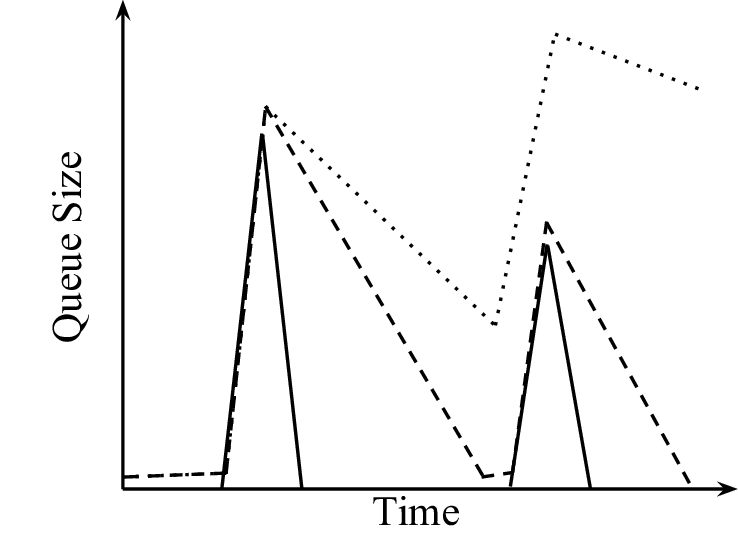
\includegraphics[width=0.4\linewidth]{QueueStacked}
\caption{
Example of network queueing during \ac{DGI} operation. \ac{DGI} modules are semi-synchronous, and create bursty traffic on the network.
When there is no other traffic on the network (solid line), the bursty traffic causes a large number of packets to queue quickly, but the queue empties at a similar rate.
With background traffic (dashed line), the bursty traffic causes a large number of packets to be queued suddenly. More packets arrive continuously, causing the queue to drain off more slowly.
When the background traffic reaches a certain threshold (dotted line), the queue does not empty before the next burst occurs. When this happens, messages will not be delivered in time, and the queue will completely fill.
}
\label{fig:queue-types}
\end{figure}

For this work, the algorithm from \cite{JOURNAL} was used.
This algorithm has a higher message complexity when in a group than the Garcia-Molina algorithm it is based on.
However, it does possess a desirable memoryless property that makes it easy to analyze.
This work uses an improved version of the algorithm which removes the restrictions in \cite{JOURNAL} where only one process could become the leader.

\subsubsection{Soft \ac{ECN}.}

A soft \ac{ECN} message indicates the network has reached a level of congestion where the router suspects processes will not be able to meet their real time requirements.
The soft \ac{ECN} message encourages the \ac{DGI} processes to reduce the number of messages they send to reduce the amount of congestion they contribute to the network, and to allow for reliable distribution techniques to have additional time to deliver messages (since fewer messages are being sent).
In the case of potential congestion, the group management module can reduce its traffic bursts by disabling elections during the congestion.
When the elections are disabled, messages for group management are only sent to members of the group.
Processes do not seek out better or other leaders to merge with.
As a consequence, the message complexity for processes responding to the congestion notification reduces from $O(n^2)$ to $O(n)$.

\subsubsection{Hard \ac{ECN}.}

In a hard \ac{ECN} scenario, the router will have determined congestion has reached a threshold where the real-time processes will soon not be able to meet their deadlines.
In this scenario, the real-time process will likely split its group.
In an uncontrolled situation, the split will be random.
It is therefore desirable when this level of traffic is reached to split the group.
Splitting the group reduces the number of messages sent across the router for modules with $O(n^2)$ (where $n$ is the number of processes in the original group) message complexity.
For larger groups, splitting them provides a significant savings in the number of messages that must be queued by the router, especially since the traffic is very bursty.

\begin{figure}
\centering
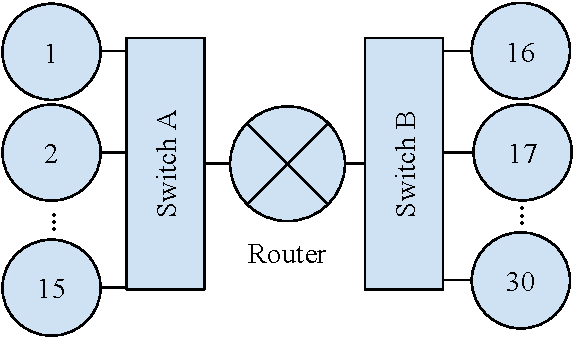
\includegraphics[width=0.35\textwidth]{NetworkLayout}
\caption{Example of process organization used in this paper. Two groups of processes are connected by a router.} \label{fig:network-layout}
\end{figure}

Suppose a network like one depicted in Figure \ref{fig:network-layout}, where processes are divided by a router.
In Figure \ref{fig:network-layout}, there are $n$ processes on one side of the network and $m$ on the other.
In normal operation the omission-modelable algorithm has an $O(n^2)$ message complexity.
In Soft \ac{ECN} maintenance mode, the reduced number of messages reduces the complexity to $O(n)$ by disabling elections.

During elections (and with each group update) the leader distributes a fallback configuration that will coordinate the division of the groups during intense congestion.
When the \ac{ECN} notification is received the processes will halt all current group management operations and enter a splitting mode where they switch to the fallback configuration.
The leader of the group distributes a fallback notification to ensure all processes in the group apply their new configuration. 
The complexity of distributing the notification is linear $O(n)$ and processes that already received the notification will have halted their communication.
This approach will ideally avoid the burst/drain phenomena from figure \ref{fig:queue-types}.

The design of the fallback configuration can be created to optimize various factors.
These factors include cyber considerations, such as the likely network path the processes in the group will use to communicate.
By selecting the group around the network resources, the group can be selected to minimize the amount of traffic that crosses the congested links in the future.
Additionally, considerations from the physical network can be considered.
Fallback groups can be created to ensure they can continue to facilitate the needs of the members.
This can take into the consideration the distribution of supply and demand processes in the current group.
By having a good mix of process types in the fallback group the potential for work can remain high.

\subsection{Cyber-Physical System}

For a real-time \ac{CPS}, message delays could affect coordinated actions.
As result, these actions may not happen at the correct moments or at all.
Since the two-army problem prevents any process from being entirely certain a coordinated action will happen in concert, problems arising from delay or omission of messages is of particular interest.
In particular, we are interested in the scenario from \cite{HARINI}, where only half of a power migration is performed.
Other power management algorithms could have similar effects on the power system based on this idea of a process performing an action that is not compensated for by other processes.

\subsubsection{Soft \ac{ECN}.}

In a soft congestion notification mode, the process being informed of the congestion can reduce its affect on the congestion by changing how often it generates bursty traffic.
Processes running the load balancing algorithm make several traffic bursts when they exchange state information and prepare migrations.
As shown before, if the interval between these bursts is not sufficient for the queue to drain before the next burst occurs, then critical, overwhelming congestion occurs.
Since the schedule of the \ac{DGI} is fixed at run-time processes cannot simply extend the duration of the load balancing execution phase.
However, on notification from the leader, the process can, instead, reduce the number of migrations to increase the message delivery interval.
This notification to reduce the schedule originates from the coordinator as part of the message exchange necessary for the process to remain in the group.
Every process in the group must receive this message to participate in load balancing, ensuring all processes remain on the same real-time schedule.
Using this approach, the amount of traffic generated is unchanged but the time period a process waits for the messages to be distributed is increased.

\subsubsection{Hard \ac{ECN}.}

When the \ac{DGI} process receives a hard congestion notification, the processes switch to a predetermined fallback configuration.
This configuration creates a cyber partition.
By partitioning the network, the number of messages sent by applications with $O(n^2)$ message complexity can be reduced significantly.
Each migration of load balancing algorithm begins with an $O(n^2)$ message burst and so benefits from the reduced group size created by the partition.

Suppose there is a network like the in Figure \ref{fig:network-layout} with $n$ processes on one half and $m$ on the other.
The number of messages sent across the router for the undivided group is of the order $2mn$ as the $n$ processes on side A send a message to the $m$ on side B and vice-versa.
Let $i_{1}$ and $j_{1}$ be the number of processes from side A and side B (respectively) in the first group created by the partition.
Let $i_{2}$ and $j_{2}$ be the number of processes in the second group created by the partition under the same circumstances of $i_1$ and $j_1$.
The number of messages sent that pass through the router, is then 

\begin{equation}
2 i_{1} j_{1} + 2 i_{2} j_{2}
\end{equation}

For an arbitrary group division, the following can be observed.
Suppose $i_{1}$ and $j_{2}$ are the cardinality of two arbitrarily chosen sets of processes from side A and side B respectively.
Following the same cut requirements as before:

\begin{equation}
i_2 = n - i_1 \text{ and } j_2 = m - j_1
\end{equation}

The the number of messages that must pass through the router for this cut is:

\begin{equation}
2 i_{1} j_{1} + 2 (n-i_{1}) (m-j_{1})
\end{equation}

The benefits of the cut are minimized when $i_1$ and $j_1$ are $\frac{n}{2}$ and $\frac{m}{2}$:

\begin{equation}
2( 2 \frac{mn}{4} + mn - \frac{mn}{2} - \frac{mn}{2}) = mn
\end{equation}

Which is a reduction of half as many messages.
For systems with a large number of participating processes this represents a significant reduction in the number of messages sent across the router.
As a consequence, this further extends the delivery window for processes sending messages.

%\subsection{Relation To Omission Model}
%
%The synchronization of clocks in the environment is assumed to be normally distributed around a true time value provided by the simulation.
%The shape of the curve created by plotting the queue resembles that of the \ac{CDF} of the normal distribution, noted $F(x)$.
%A simple description of the traffic behavior can then be described in terms of that curve.
%First, observe that when the queue hits a specific threshold, even if the queue is drained at an optimal rate, the $n$th queued packed will not be delivered in time:
%
%\begin{equation}
%Qsize - min(Qsize, (DequeueRate * \Delta t)) \geq 0
%\label{eq:origin}
%\end{equation}
%
%Where $\Delta t$ is the deadline for the message to be delivered.
%If the size of the queue exceeds the number of messages that can be delivered before $\Delta t$ passes, some messages will not be delivered.
%The size of the queue during the message bursts created by the DGI depends on the message complexity of the algorithm, the number of messages already in the queue, the other traffic on the network, and any replies that also have to be delivered in that interval.
%Therefore, let $c$ represent the rate that traffic is generated by other processes.
%Let $init_q$ represent the number of messages in the queue at the start of a burst. 
%Let $init_m$ represent the number of messages sent in the beginning of the burst.
%Let $resp$ represent the number of messages sent in response to the burst that must still be delivered before $\Delta t$ passes.
%We can then express $Qsize$ as two parts:
%
%\begin{equation}
%Qsize = Burst + Obligations
%\end{equation}
%
%Where $Burst$ takes the form of the \ac{CDF} for the normal distribution:
%
%\begin{equation}
%Burst = init_m * F(x)  
%\end{equation}
%
%\begin{equation}
%Obligations = c * \Delta t + init_q + resp
%\end{equation}
%
%From this we can derive the equation:
%
%\begin{equation}
%F(x) \geq \frac{DequeueRate * \Delta t - c * \Delta t - init_q - resp}{init_m}
%\label{eq:prob-est}
%\end{equation}
%
%Where, from Equation \ref{eq:origin}, $DequeueRate * \Delta t$ is less than or equal to the number of messages in the queue. 
%Solving for $F(x)$ gives a worst case estimate of the omission rate for a specific algorithmic or network circumstance.
%$DequeueRate$ is affected by the amount of traffic in the system. 
%It should be obvious a greater amount of background traffic corresponds to a greater average queue size.
%From an relationship between the background traffic and the average queue size and the results presented in \cite{JOURNAL}, Equation \ref{eq:prob-est} can be used to select the ECN parameters.
